\documentclass[12pt, fullpage,letterpaper]{article}

\usepackage[margin=1in]{geometry}
\usepackage{url}
\usepackage{amsmath}
\usepackage{amssymb}
\usepackage{xspace}
\usepackage{graphicx}
\usepackage{hyperref}
\usepackage{cancel}
%\usepackage{graphicx}
%\usepackage{subfig}
\usepackage{hyperref}
\usepackage{xcolor}
\usepackage{ulem}
\usepackage{cancel}
\usepackage{float}

\def\red{\color{black!30!red}}
\def\blue{\color{blue}}
\def\blackblue{\color{black!40!blue}}




\newcommand{\semester}{Spring 2022}
\newcommand{\assignmentId}{3}
\newcommand{\releaseDate}{15 Mar, 2022}
\newcommand{\dueDate}{11:59pm, 29 Mar, 2022}
\newcommand\independent{\protect\mathpalette{\protect\independenT}{\perp}}
\def\independenT#1#2{\mathrel{\rlap{$#1#2$}\mkern2mu{#1#2}}}

\newcommand{\bx}{{\bf x}}
\newcommand{\bw}{{\bf w}}

\title{CS 6190: Probabilistic Machine Learning \semester}
\author{Homework \assignmentId}
\date{Handed out: \releaseDate\\
  Due: \dueDate}

\begin{document}
\maketitle

% Math commands by Thomas Minka
\newcommand{\var}{{\rm var}}
\newcommand{\Tr}{^{\rm T}}
\newcommand{\vtrans}[2]{{#1}^{(#2)}}
\newcommand{\kron}{\otimes}
\newcommand{\schur}[2]{({#1} | {#2})}
\newcommand{\schurdet}[2]{\left| ({#1} | {#2}) \right|}
\newcommand{\had}{\circ}
\newcommand{\diag}{{\rm diag}}
\newcommand{\invdiag}{\diag^{-1}}
\newcommand{\rank}{{\rm rank}}
% careful: ``null'' is already a latex command
\newcommand{\nullsp}{{\rm null}}
\newcommand{\tr}{{\rm tr}}
\renewcommand{\vec}{{\rm vec}}
\newcommand{\vech}{{\rm vech}}
\renewcommand{\det}[1]{\left| #1 \right|}
\newcommand{\pdet}[1]{\left| #1 \right|_{+}}
\newcommand{\pinv}[1]{#1^{+}}
\newcommand{\erf}{{\rm erf}}
\newcommand{\hypergeom}[2]{{}_{#1}F_{#2}}

% boldface characters
\renewcommand{\a}{{\bf a}}
\renewcommand{\b}{{\bf b}}
\renewcommand{\c}{{\bf c}}
\renewcommand{\d}{{\rm d}}  % for derivatives
\newcommand{\e}{{\bf e}}
\newcommand{\f}{{\bf f}}
\newcommand{\g}{{\bf g}}
\newcommand{\h}{{\bf h}}
%\newcommand{\k}{{\bf k}}
% in Latex2e this must be renewcommand
\renewcommand{\k}{{\bf k}}
\newcommand{\m}{{\bf m}}
\newcommand{\mb}{{\bf m}}
\newcommand{\n}{{\bf n}}
\renewcommand{\o}{{\bf o}}
\newcommand{\p}{{\bf p}}
\newcommand{\q}{{\bf q}}
\renewcommand{\r}{{\bf r}}
\newcommand{\s}{{\bf s}}
\renewcommand{\t}{{\bf t}}
\renewcommand{\u}{{\bf u}}
\renewcommand{\v}{{\bf v}}
\newcommand{\w}{{\bf w}}
\newcommand{\x}{{\bf x}}
\newcommand{\y}{{\bf y}}
\newcommand{\z}{{\bf z}}
%s\newcommand{\l}{\boldsymbol{l}}
\newcommand{\A}{{\bf A}}
\newcommand{\B}{{\bf B}}
\newcommand{\C}{{\bf C}}
\newcommand{\D}{{\bf D}}
\newcommand{\E}{{\bf E}}
\newcommand{\F}{{\bf F}}
\newcommand{\G}{{\bf G}}
\renewcommand{\H}{{\bf H}}
\newcommand{\I}{{\bf I}}
\newcommand{\J}{{\bf J}}
\newcommand{\K}{{\bf K}}
\renewcommand{\L}{{\bf L}}
\newcommand{\M}{{\bf M}}
\newcommand{\N}{\mathcal{N}}  % for normal density
\newcommand{\Dcal}{\mathcal{D}}  % for normal density

%\newcommand{\N}{{\bf N}}
\renewcommand{\O}{{\bf O}}
\renewcommand{\P}{{\bf P}}
\newcommand{\Q}{{\bf Q}}
\newcommand{\R}{{\bf R}}
\renewcommand{\S}{{\bf S}}
\newcommand{\T}{{\bf T}}
\newcommand{\U}{{\bf U}}
\newcommand{\V}{{\bf V}}
\newcommand{\W}{{\bf W}}
\newcommand{\X}{{\bf X}}
\newcommand{\Y}{{\bf Y}}
\newcommand{\Z}{{\bf Z}}

% this is for latex 2.09
% unfortunately, the result is slanted - use Latex2e instead
%\newcommand{\bfLambda}{\mbox{\boldmath$\Lambda$}}
% this is for Latex2e
\newcommand{\bfLambda}{\boldsymbol{\Lambda}}

% Yuan Qi's boldsymbol
\newcommand{\bsigma}{\boldsymbol{\sigma}}
\newcommand{\balpha}{\boldsymbol{\alpha}}
\newcommand{\bpsi}{\boldsymbol{\psi}}
\newcommand{\bphi}{\boldsymbol{\phi}}
\newcommand{\boldeta}{\boldsymbol{\eta}}
\newcommand{\Beta}{\boldsymbol{\eta}}
\newcommand{\btau}{\boldsymbol{\tau}}
\newcommand{\bvarphi}{\boldsymbol{\varphi}}
\newcommand{\bzeta}{\boldsymbol{\zeta}}

\newcommand{\blambda}{\boldsymbol{\lambda}}
\newcommand{\bLambda}{\mathbf{\Lambda}}
\newcommand{\bOmega}{\mathbf{\Omega}}
\newcommand{\bomega}{\mathbf{\omega}}
\newcommand{\bPi}{\mathbf{\Pi}}

\newcommand{\btheta}{\boldsymbol{\theta}}
\newcommand{\bpi}{\boldsymbol{\pi}}
\newcommand{\bxi}{\boldsymbol{\xi}}
\newcommand{\bSigma}{\boldsymbol{\Sigma}}

\newcommand{\bgamma}{\boldsymbol{\gamma}}
\newcommand{\bGamma}{\mathbf{\Gamma}}

\newcommand{\bmu}{\boldsymbol{\mu}}
\newcommand{\1}{{\bf 1}}
\newcommand{\0}{{\bf 0}}

% \newcommand{\comment}[1]{}

\newcommand{\bs}{\backslash}
\newcommand{\ben}{\begin{enumerate}}
\newcommand{\een}{\end{enumerate}}

 \newcommand{\notS}{{\backslash S}}
 \newcommand{\nots}{{\backslash s}}
 \newcommand{\noti}{{\backslash i}}
 \newcommand{\notj}{{\backslash j}}
 \newcommand{\nott}{\backslash t}
 \newcommand{\notone}{{\backslash 1}}
 \newcommand{\nottp}{\backslash t+1}
% \newcommand{\notz}{\backslash z}

\newcommand{\notk}{{^{\backslash k}}}
%\newcommand{\noti}{{^{\backslash i}}}
\newcommand{\notij}{{^{\backslash i,j}}}
\newcommand{\notg}{{^{\backslash g}}}
\newcommand{\wnoti}{{_{\w}^{\backslash i}}}
\newcommand{\wnotg}{{_{\w}^{\backslash g}}}
\newcommand{\vnotij}{{_{\v}^{\backslash i,j}}}
\newcommand{\vnotg}{{_{\v}^{\backslash g}}}
\newcommand{\half}{\frac{1}{2}}
\newcommand{\msgb}{m_{t \leftarrow t+1}}
\newcommand{\msgf}{m_{t \rightarrow t+1}}
\newcommand{\msgfp}{m_{t-1 \rightarrow t}}

\newcommand{\proj}[1]{{\rm proj}\negmedspace\left[#1\right]}
\newcommand{\argmin}{\operatornamewithlimits{argmin}}
\newcommand{\argmax}{\operatornamewithlimits{argmax}}

\newcommand{\dif}{\mathrm{d}}
\newcommand{\abs}[1]{\lvert#1\rvert}
\newcommand{\norm}[1]{\lVert#1\rVert}

%miscellaneous symbols
\newcommand{\ie}{{{i.e.,}}\xspace}
\newcommand{\eg}{{{\em e.g.,}}\xspace}
\newcommand{\EE}{\mathbb{E}}
\newcommand{\VV}{\mathbb{V}}
\newcommand{\sbr}[1]{\left[#1\right]}
\newcommand{\rbr}[1]{\left(#1\right)}
\newcommand{\cmt}[1]{}



\footnotesize
	\begin{itemize}
		\item You are welcome to talk to other members of the class about
		the homework. I am more concerned that you understand the
		underlying concepts. However, you should write down your own
		solution. Please keep the class collaboration policy in mind.
		
		\item Feel free discuss the homework with the instructor or the TAs.
		
		\item Your written solutions should be brief and clear. You need to
		show your work, not just the final answer, but you do \emph{not}
		need to write it in gory detail. Your assignment should be {\bf no
			more than 10 pages}. Every extra page will cost a point.
		
		\item Handwritten solutions will not be accepted.
		
		\item The homework is due by \textbf{midnight of the due date}. Please submit
		the homework on Canvas.
	\end{itemize}



\section*{Analytical problems [100 points + 40 bonus]}	
\label{sec:q1}
%1. show Jeffery's prior for Gaussian
%2. show Jeffern's prior for Poisson 
\begin{enumerate}
\item~[13 points] The joint distribution over three binary variables are given in Table \ref{tb:abc}. Show by direct evaluation that this distribution has the property that $a$ and $b$ are marginally dependent, so that $p(a, b) \neq p(a)p(b)$, but that they become independent conditioned on $c$, \ie  $p(a,b|c) = p(a|c)p(b|c)$. 
\begin{table}
	\centering
	\begin{tabular}{c|c|c|c}
		\hline
		a & b & c  & p(a,b,c)\\
		\hline
		0 & 0 & 0 & 0.192\\
		0 & 0 & 1 & 0.144\\
		0 & 1 & 0 & 0.048\\
		0 & 1 & 1 & 0.216\\
	    1 & 0 & 0 & 0.192\\
	    1 & 0 & 1  & 0.064\\
	    1 & 1 & 0 & 0.048\\
	    1 & 1 & 1 & 0.096\\
	    \hline
	\end{tabular}
\caption{Joint distribution of $a,b,c$.} \label{tb:abc}
\end{table}
{\bf \red Answer:}{\blackblue 
Let us first comlute $p(a),p(b) p(a,b), p(a|c), p(b|c)$.
\begin{table}
	\centering
	\begin{tabular}{||c|c||}
		\hline
		a & p(a)\\
		\hline
		0 & 0.6\\
		1 & 0.4\\
	    \hline
	\end{tabular}
	\quad\quad  
	\begin{tabular}{||c|c||}
		\hline
		b & p(b)\\
		\hline
		0 & 0.592\\
		1 & 0.408\\
	    \hline
	\end{tabular}
	\quad\quad  
	\begin{tabular}{||c|c||}
		\hline
		c & p(c)\\
		\hline
		0 & 0.48\\
		1 & 0.52\\
	    \hline
	\end{tabular}
	\quad\text{and}\quad  
	\begin{tabular}{||c|c|c||}
		\hline
		$a$ & $b$ & $p(a,b)$\\
		\hline
		0 & 0 & 0.336\\
		0 & 1 & 0.264\\
		1 & 0 & 0.256\\
		1 & 1 & 0.144\\
	    \hline
	\end{tabular}
\caption{Distributions of $p(a),p(b), p(c)$ and $p(a,b)$.} \label{tb:joint}
\end{table}
In view of Table~\ref{tb:joint}, we can see that 
$$p(a=0)p(b=0) \neq p(a=0,b=0)$$ which indicates that $a$ and $b$ are not independent. 
Also, Table~\ref{tb:abgivenc} showes that for each value of $a,b,c$, we have the equality $p(a|c)p(b|c) = p(a,b|c)$ which means $a$ and $b$ are conditioned on $c$.

\begin{table}
	\centering
	\begin{tabular}{||c|c|c||}
		\hline
		$a$ & $c$ & $p(a|c)$\\
		\hline
		0 & 0 & 0.5\\
		1 & 0 & 0.5\\
		\hline
		\hline
		0 & 1 & 0.6923\\
		1 & 1 & 0.3076\\
	    \hline
	\end{tabular}
	\quad\text{and}\quad  
		\begin{tabular}{||c|c|c||}
		\hline
		$b$ & $c$ & $p(b|c)$\\
		\hline
		\hline
		0 & 0 & 0.8\\
		1 & 0 & 0.2\\
		\hline
		0 & 1 & 0.4\\
		1 & 1 & 0.6\\
	    \hline
	\end{tabular}
	\quad\text{and}\quad  
		\begin{tabular}{||c|c||c||c||}
		\hline
		$a$ & $b$ & $c$ & $p(a,b|c)$\\
		\hline
		\hline
		0 & 0 & 0 & 0.4\\
		0 & 1 & 0 & 0.1\\
		1 & 0 & 0 & 0.4\\
		1 & 1 & 0 & 0.1\\
		\hline
		0 & 0 & 1 & 0.2769\\
		0 & 1 & 1 & 0.4154\\
		1 & 0 & 1 & 0.1232\\
		1 & 1 & 1 & 0.18462\\
	    \hline
	\end{tabular}
\caption{Conditional distributions of $a|c$ and $b|c$.} \label{tb:abgivenc}
\end{table}
}

\item~[12 points] Using the $d$-separation algorithm/criterion (Bayes ball algorithm) to show that the conditional distribution for a node $x$ in a directed graph, conditioned on all of the nodes in its Markov blanket, is independent of the remaining variables in the graph.\\
{\bf \red Answer: }{\blackblue 
Let $x$ be an arbitrary vertex in an acyclic graph $T$ and denotes its Markov blanket $MB(x)$. 
Assume that $P=xz_1z_2\cdots z_m=y$ is a path from $x$ to a vertex $y$ outside of $MB(x)$.
In view of the $d$-separation $d$-separation criterion, to prove the desired assertion, we need to prove that the path $P$ is blocked. 
Distinguish the following cases:
\begin{itemize}
\item[(1)] {\bf $z_1$ is a chid of $x$.} In this case, if $z_2$ is a child of $z_1$, then the arrows on the path meet the vertex $z_1$ in head-to-tail. Since $z_1$ is in $MB(x)$, the path is blocked. If $z_2$ is a parent of $z_1$, then $z_2\in MB(x)$ (thus $z_2\neq y$) and the arrows on the path meet the vertex $z_2$ either in head-to-tail or tail-to-tail (depending on whether $z_3$ is a parent of a child of $z_2$) which implies that the path is blocked. 
\item[(2)] {\bf $z_1$ is a parent of $x$.} In this case, if $z_2$ is a child of $z_1$, then the arrows on the path meet the vertex $z_1$ in tail-to-tail and if 
$z_2$ is a parent of $z_1$, then the arrows on the path meet the vertex $z_1$ in head-to-tail. Therefore, since $z_1$ is in $MB(x)$, the path is blocked. \end{itemize}

}


\begin{figure}[h]
\centering
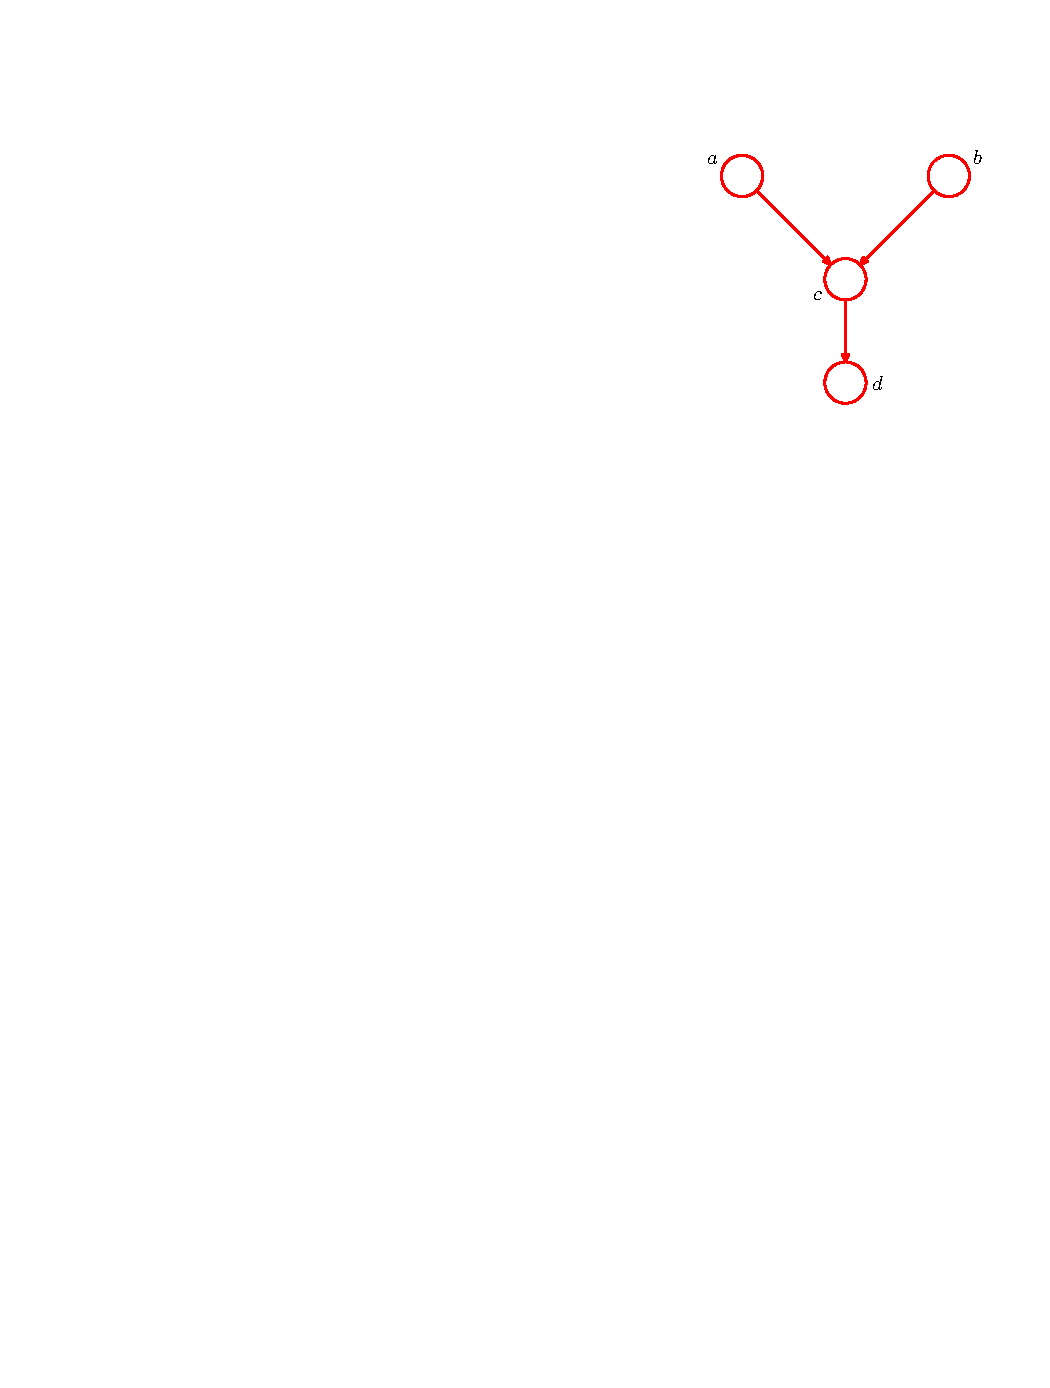
\includegraphics[width=0.3\linewidth]{./fig1.pdf} 
\caption{Graphical model.} \label{fig:graph}
\end{figure}

\item~[15 points] See the graphical model in Figure \ref{fig:graph}. Recall what we have discussed in the class. Show that $a \independent b | \emptyset $. Suppose we have observed the variable $d$. Show that in general $a \cancel{ \independent} b | d$.\\
{\bf \red Answer: }{\blackblue 
According to the graphical model, 
$$p(a,b,c,d)=p(a)p(b)p(c|a,b)p(d|c).$$
Therefore, 
\begin{align*}
p(a,b) & = \int_{c,d}p(a)p(b)p(c|a,b)p(d|c)\d c\d d\\
& = p(a)p(b)\int{c}p(c|a,b)\underbrace{\int_{d}p(d|c)\d d}_{= 1}\d c\\
& = p(a)p(b)\underbrace{\sum_{c}p(c|a,b)}_{=1}\d c = p(a)p(b)
\end{align*}
which implies that $a \independent b | \emptyset$. 
To prove $a \cancel{ \independent} b | d$, 
\begin{align*}
p(a,b|d) & = \frac{p(a,b,d)}{p(d)}\\
& = \frac{\int_{c} p(a,b,c,d)\d c}{p(d)}\\
& = \frac{\int_{c}p(a)p(b)p(c|a,b)p(d|c)\d c}{p(d)}\\
& = \frac{p(a)p(b)\int_{c}p(c|a,b)p(d|c)\d c}{p(d)}.
\end{align*}
However, $\int_{c}p(c|a,b)p(d|c)\d c$ generally cannot be decompose into $m(a,d)\times n(b,d)$ and consequently, 
$$p(a,b|d) \neq p(a|d)p(b|d).$$
}
\item~[10  points] Convert the directed graphical model in Figure \ref{fig:graph} into an undirected graphical model. Draw the structure and write down the definition of the potential functions. \\
{\bf \red Answer: }{\blackblue 
The converted undirected graphical model is shown in Figure~\ref{fig:graph2_und}. 
In view of the directed graphical model in Figure \ref{fig:graph}, we obtain  
$p(a,b,c,d) = p(a)p(b)p(c|a,b)p(d|c)$. We can rewrite it as  
$$p(a,b,c,d) = \underbrace{p(a)p(b)p(c|a,b)}_{\psi_1(a,b,c)}\underbrace{p(d|c)}_{\psi_2(c,d)}$$
and set $Z=1$. Therefore, 
$$p(a,b,c,d) = \psi_1(a,b,c)\psi_2(c,d),$$
where $\psi_1(a,b,c)=p(a)p(b)p(c|a,b)$ and $\psi_2(c,d)=p(d|c).$
\begin{figure}[h]
	\centering
	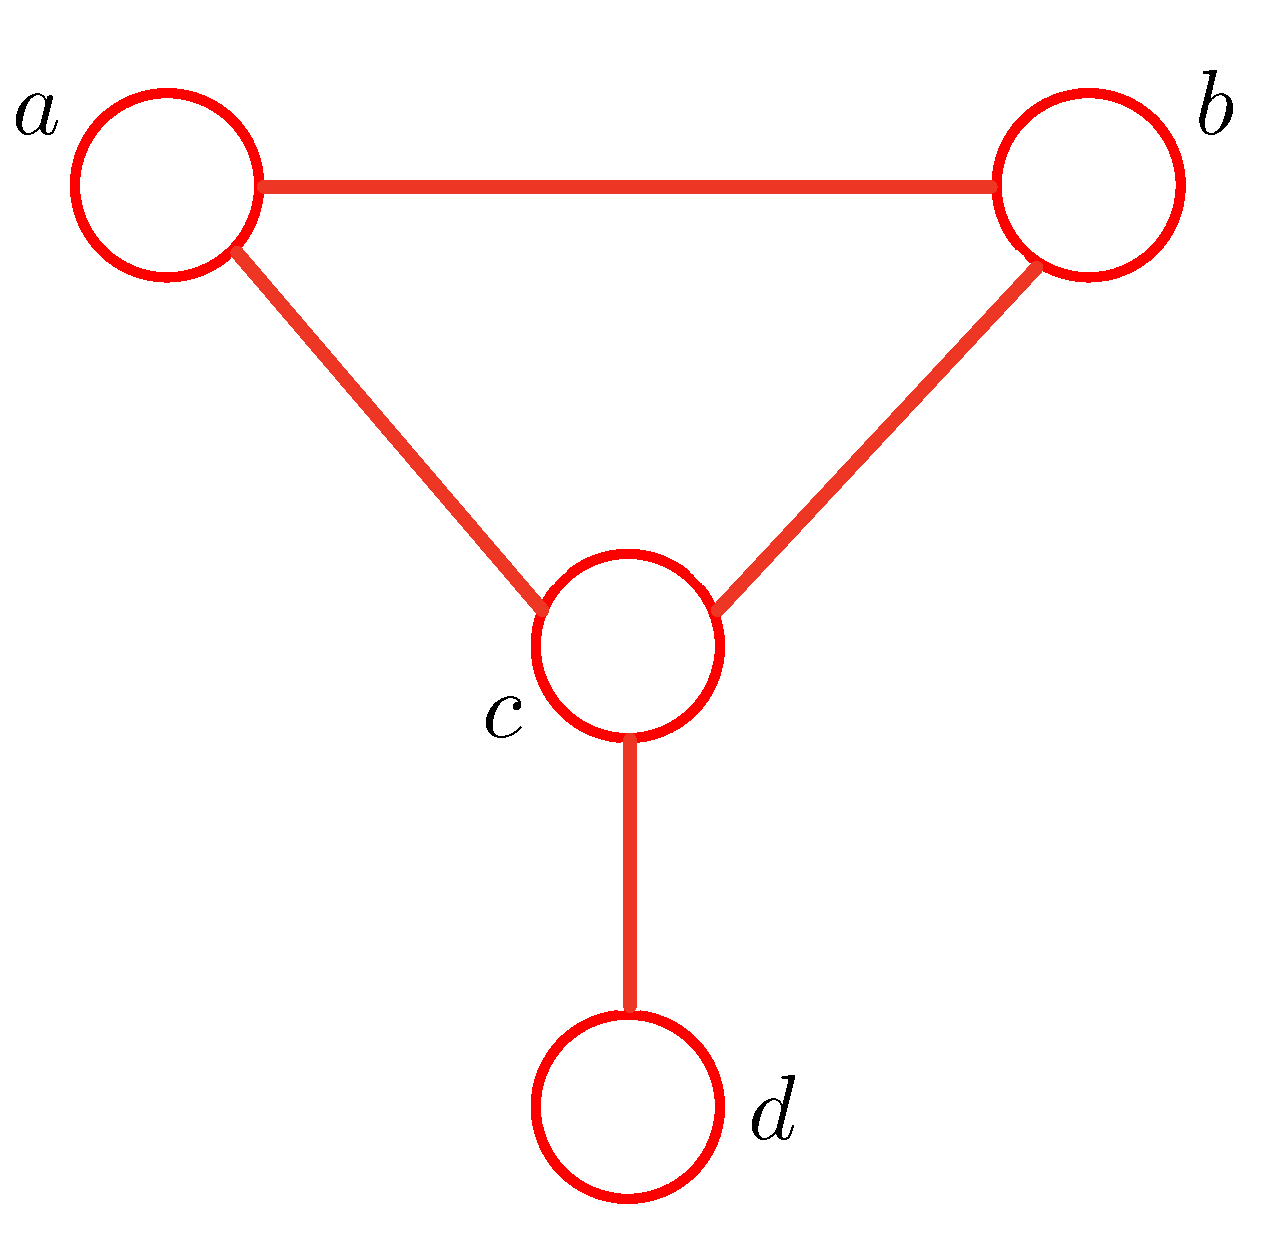
\includegraphics[width=0.4\linewidth]{./fig1_und.pdf} 
	\caption{Undirected graphical model of Figure \ref{fig:graph}} \label{fig:graph2_und}
\end{figure}
}


\item~[15 points] Write down every step of the sum-product algorithm for the graphical model shown in Figure \ref{fig:graph2}. Note that you need to first choose a root node, and write down how to compute each message. Once all your messages are ready, please explain how to compute the marginal distribution $p(x_4, x_5)$.\\
{\bf \red Answer: }{\blackblue 
We set $x_4$ to be the root. We have three leaf nodes $x_1$, $x_3$, and $f_d$. 
Also, note that unnormalized joint distribution is given by $$\tilde{p}(x_1,x_2,x_3,x_4,x_5) = f_a(x_1,x_2,x_3)f_b(x_2,x_4)f_c(x_4,x_5)f_d(x_5).$$
\begin{itemize}
\item[$\bullet$] {\bf Propagation messages from the leaf nodes out to the root node.}\\ 
We have the following eight messages. 
\begin{equation}
\mu_{f_d\rightarrow x_5}(x_5) = f_d(x_5)
\end{equation}
\begin{equation}
\mu_{x_5\rightarrow f_c}(x_5) = \prod_{l\in ne(x_5)\setminus f_c}\mu_{f_l\rightarrow x_5}(x_5) = f_d(x_5)
\end{equation}

\begin{align}
\mu_{f_c\rightarrow x_4}(x_4) & = \sum_{x_5}f_c(x_4,x_5)\mu_{x_5\rightarrow f_c}(x_5)\nonumber \\
& = \sum_{x_5}f_c(x_4,x_5)f_d(x_5)
\end{align}



\begin{equation}
\mu_{x_1\rightarrow f_a}(x_1) = 1
\end{equation}
\begin{equation}
\mu_{x_3\rightarrow f_a}(x_3) = 1
\end{equation}

\begin{align}
\mu_{f_a\rightarrow x_2}(x_2) & =  \sum_{x_1,x_3}f_a(x_1,x_2,x_3)\mu_{x_1\rightarrow f_a}(x_1)\mu_{x_3\rightarrow f_a}(x_3) \nonumber \\
& = \sum_{x_1,x_3}f_a(x_1,x_2,x_3)
\end{align}

\begin{align}
\mu_{x_2\rightarrow f_b}(x_2) 
&=  \prod_{l\in ne(x_2)\setminus f_b}\mu_{f_l\rightarrow x_2}(x_2)\nonumber \\
& = \mu_{f_a\rightarrow x_2}(x_2) \\
& = \sum_{x_1,x_3}f_a(x_1,x_2,x_3)\nonumber 
\end{align}

\begin{align}
\mu_{f_b\rightarrow x_4}(x_4) & = \sum_{x_2}f_b(x_2,x_4)\mu_{x_2\rightarrow f_b}(x_2)\nonumber \\
& = \sum_{x_2}f_b(x_2,x_4)\sum_{x_1,x_3}f_a(x_1,x_2,x_3)
\end{align}

\item[$\bullet$]{\bf Propagation messages from the root node out to the leaf nodes.}
\begin{align}
\mu_{x_4\rightarrow f_c}(x_4) 
&=  \prod_{l\in ne(x_4)\setminus f_c}\mu_{f_l\rightarrow x_4}(x_4)\nonumber \\
& = \mu_{f_b\rightarrow x_4}(x_4)\\
& = \sum_{x_2}f_b(x_2,x_4)\sum_{x_1,x_3}f_a(x_1,x_2,x_3)
\end{align}

\begin{align}
\mu_{f_c\rightarrow x_5}(x_5) & =\sum_{x_4}f_c(x_4,x_5)\mu_{x_4\rightarrow f_c}(x_4)\nonumber \\
%& = \sum_{x_4}f_c(x_4,x_5)\mu_{x_4\rightarrow f_c}(x_4)\\
& = \sum_{x_4}f_c(x_4,x_5)\sum_{x_2}f_b(x_2,x_4)\sum_{x_1,x_3}f_a(x_1,x_2,x_3)
\end{align}

\begin{align}
\mu_{x_5\rightarrow f_d}(x_5) 
&=  \prod_{l\in ne(x_5)\setminus f_d}\mu_{f_l\rightarrow x_5}(x_5)\nonumber \\
& = \mu_{f_c\rightarrow x_5}(x_5)\\
& = \sum_{x_4}f_c(x_4,x_5)\sum_{x_2}f_b(x_2,x_4)\sum_{x_1,x_3}f_a(x_1,x_2,x_3)\nonumber
\end{align}


\begin{align}
\mu_{x_4\rightarrow f_b}(x_4) 
&=  \prod_{l\in ne(x_4)\setminus f_b}\mu_{f_l\rightarrow x_4}(x_4)\nonumber \\
& = \mu_{f_c\rightarrow x_4}(x_4)\\
& = \sum_{x_5}f_c(x_4,x_5)f_d(x_5)\nonumber
\end{align}

\begin{align}
\mu_{f_b\rightarrow x_2}(x_2) & =\sum_{x_4}f_b(x_2,x_4)\mu_{x_4\rightarrow f_b}(x_4)\nonumber \\
& = \sum_{x_4}f_b(x_2,x_4)\sum_{x_5}f_c(x_4,x_5)f_d(x_5)
\end{align}


\begin{align}
\mu_{x_2\rightarrow f_a}(x_2) 
&=  \prod_{l\in ne(x_2)\setminus f_a}\mu_{f_l\rightarrow x_2}(x_2)\nonumber \\
& = \mu_{f_b\rightarrow x_2}(x_2)\\
& =  \sum_{x_4}f_b(x_2,x_4)\sum_{x_5}f_c(x_4,x_5)f_d(x_5)\nonumber
\end{align}


\begin{align}
\mu_{f_a\rightarrow x_1}(x_1) & =\sum_{x_2,x_3}f_a(x_1,x_2,x_3)\mu_{x_2\rightarrow f_a}(x_2)\mu_{x_3\rightarrow f_a}(x_3)\nonumber \\
& =\sum_{x_2,x_3}f_a(x_1,x_2,x_3)\sum_{x_4}f_b(x_2,x_4)\sum_{x_5}f_c(x_4,x_5)f_d(x_5)
\end{align}


\begin{align}
\mu_{f_a\rightarrow x_3}(x_3) & =\sum_{x_1,x_2}f_a(x_1,x_2,x_3)\mu_{x_1\rightarrow f_a}(x_2)\mu_{x_2\rightarrow f_a}(x_3)\nonumber \\
& =\sum_{x_1,x_2}f_a(x_1,x_2,x_3) \sum_{x_4}f_b(x_2,x_4)\sum_{x_5}f_c(x_4,x_5)f_d(x_5)
\end{align}
\end{itemize}


{\bf Unnormalized Marginal $\tilde{p}(x_4,x_5)$:}\\
\begin{align*}
\tilde{p}(x_4,x_5) 
& = f_c(x_4,x_5)\mu_{f_d\rightarrow x_5}(x_5)\mu_{f_b\rightarrow x_4}(x_4)\\
& = f_c(x_4,x_5)f_d(x_5) \sum_{x_2}f_b(x_2,x_4)\sum_{x_1,x_3}f_a(x_1,x_2,x_3)
\end{align*}
Therefore,  
$$p(x_4,x_5) = \frac{\tilde{p}(x_4,x_5)}{\sum\limits_{x_4,x_5}\tilde{p}(x_4,x_5)}.$$
}
\begin{figure}[h]
	\centering
	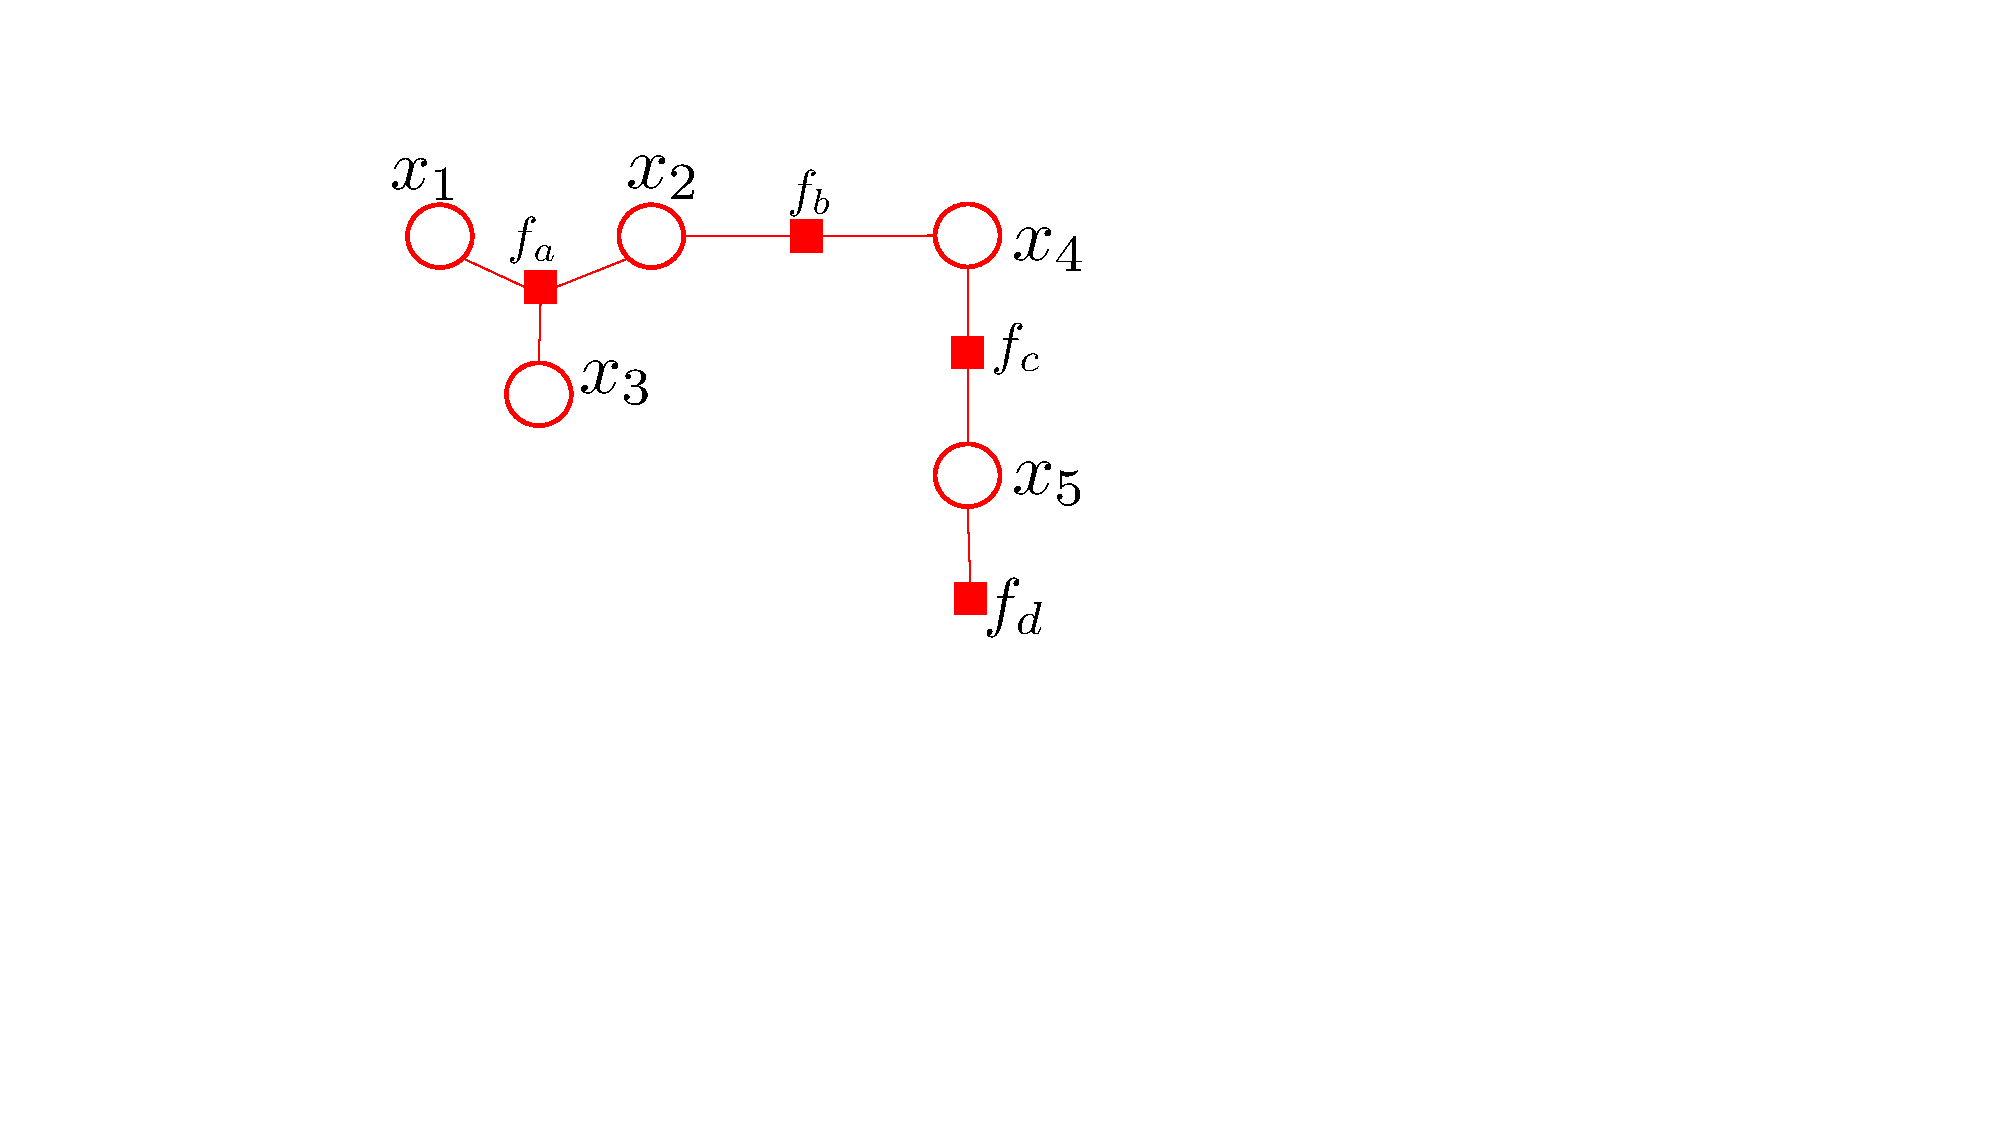
\includegraphics[width=0.2\linewidth]{./fig2.pdf} 
	\caption{Factor graph.} \label{fig:graph2}
\end{figure}


\item~[10 points] Now if $x_2$ in Figure \ref{fig:graph2} is observed, explain how to conduct the sum-product algorithm, and compute the posterior distribution $p(x_4, x_5|x_2)$.\\
{\bf \red Answer: }{\blackblue 
When $x_2=\alpha$ is observed, we can run the sum-product algorithm exactly similar to the previous question while we are keeping in mind that the range of $x_2$ is only $\{\alpha\}$. In other words, in any summation over $x_2$,  the only possible value for $x_2$ to take is $\alpha$.
Therefore, we can repeat exactly what we did in the previous question, and finally, set the range of $x_2$ to be only $\{\alpha\}$. 

{\bf Unnormalized Marginal $\tilde{p}(x_4,x_5|x_2)$:}
\begin{align*}
\tilde{p}(x_4,x_5|x_2) 
& = f_c(x_4,x_5)\mu_{f_d\rightarrow x_5}(x_5)\mu_{f_b\rightarrow x_4}(x_4)\\
& = f_c(x_4,x_5)f_d(x_5) \sum_{x_2\in\{\alpha\}}f_b(x_2,x_4)\sum_{x_1,x_3}f_a(x_1,x_2,x_3)\\
& = f_c(x_4,x_5)f_d(x_5) f_b(\alpha,x_4)\sum_{x_1,x_3}f_a(x_1,\alpha,x_3)
\end{align*}
Therefore,  
$$p(x_4,x_5|x_2) = \frac{\tilde{p}(x_4,x_5|x_2)}{\sum\limits_{x_4,x_5}\tilde{p}(x_4,x_5|x_2)}.$$
}


\item~[10 points] Suppose all the random variables in Figure \ref{fig:graph2} are discrete, and no one has been observed. Now we want to find the configuration of the $x_1, \ldots, x_5$ to maximize the joint probability. Write done every step of the max-sum algorithm to calculate the maximum joint probability and to find the corresponding configurations of each random variable. \\
{\bf \red Answer: }{\blackblue 
We set $x_4$ to be the root. We have three leaf nodes $x_1$, $x_3$, and $f_d$. 
\begin{equation}
\mu_{f_d\rightarrow x_5}(x_5) =\ln f_d(x_5)
\end{equation}
\begin{equation}
\mu_{x_5\rightarrow f_c}(x_5) = \sum_{l\in ne(x_5)\setminus f_c}\mu_{f_l\rightarrow x_5}(x_5) = \ln f_d(x_5)
\end{equation}
\begin{align}
\mu_{f_c\rightarrow x_4}(x_4) & = \max_{x_5}\big[\ln f_c(x_4,x_5) + \mu_{x_5\rightarrow f_c}(x_5)\big]\nonumber \\
& = \max_{x_5}\big[\ln f_c(x_4,x_5) +  \ln f_d(x_5)\big]\label{fcx4}\\
{\red \phi_{f_c\rightarrow x_4}(x_4)} & = {\red \arg\max_{x_5}\big[\ln f_c(x_4,x_5) +  \ln f_d(x_5)\big]}\label{phicx4}
\end{align}
\begin{equation}
\mu_{x_1\rightarrow f_a}(x_1) = 0
\end{equation}
\begin{equation}
\mu_{x_3\rightarrow f_a}(x_3) = 0
\end{equation}
\begin{align}
\mu_{f_a\rightarrow x_2}(x_2) & =  \max_{x_1,x_3}\big[\ln f_a(x_1,x_2,x_3)+ \mu_{x_1\rightarrow f_a}(x_1)+ \mu_{x_3\rightarrow f_a}(x_3)\big] \nonumber \\
& = \max_{x_1,x_3}\ln f_a(x_1,x_2,x_3)\label{fax2}\\
{\red \phi_{f_a\rightarrow x_2}(x_2)} & = {\red \arg\max_{x_1,x_3}\big[\ln f_a(x_1,x_2,x_3)\big]}\label{phiax2}
\end{align}
\begin{align}
\mu_{x_2\rightarrow f_b}(x_2) 
&=  \sum_{l\in ne(x_2)\setminus f_b}\mu_{f_l\rightarrow x_2}(x_2)\nonumber \\
& = \mu_{f_a\rightarrow x_2}(x_2) \\
& = \max_{x_1,x_3}\ln f_a(x_1,x_2,x_3)\nonumber 
\end{align}
\begin{align}
\mu_{f_b\rightarrow x_4}(x_4) & = \max_{x_2}\big[\ln f_b(x_2,x_4)+\mu_{x_2\rightarrow f_b}(x_2)\big]\nonumber \\
& = \max_{x_2}\Big[\ln f_b(x_2,x_4)+ \max_{x_1,x_3}\ln f_a(x_1,x_2,x_3)\Big]\label{fbx4}\\
{\red \phi_{f_b\rightarrow x_4}(x_4)} & = {\red \arg\max_{x_2}\big[\ln f_b(x_2,x_4)+ \max_{x_1,x_3}\ln f_a(x_1,x_2,x_3)\big]}\label{phibx4}
\end{align}
Using Eqautions (\ref{fcx4}) and (\ref{fbx4}), we obtain the maximum of log-joint probability as follows
\begin{align}\max\ln \tilde{p}(x_1,\ldots,x_5) 
& = \max\limits_{x_4}\sum_{l\in ne(x_4)}\mu_{f_l\rightarrow x_4}(x_4)\nonumber\\
& = \max\limits_{x_4}\big[\mu_{f_b\rightarrow x_4}(x_4) + \mu_{f_c\rightarrow x_4}(x_4)\big]\label{maxjoint}\\
& = \max_{x_4}\left[ \max_{x_5}\big[\ln f_c(x_4,x_5) +  \ln f_d(x_5)\big]+\max_{x_2}\big[\ln f_b(x_2,x_4)+ \max_{x_1,x_3}\ln f_a(x_1,x_2,x_3)\big]\right]\nonumber
\end{align}
{\red To find the corresponding configurations of each random variable, using \ref{maxjoint}, 
we first get $$x_4^* = \arg\max\limits_{x_4}\sum_{l\in ne(x_4)}\mu_{f_l\rightarrow x_4}(x_4).$$
Then, recursively, we obtain  
\begin{align*}
x_5^* & = \phi_{f_c\rightarrow x_4}(x_4^*)\quad\quad \text{using \ref{phicx4}}\\
x_2^* & = \phi_{f_b\rightarrow x_4}(x_4^*)\quad\quad \text{using \ref{phibx4}}\\
x_1^*,x_3^* & = \phi_{f_a\rightarrow x_2}(x_2^*)\quad\quad \text{using \ref{phiax2}}
\end{align*}
}}
\item~[\textbf{Bonus}][20 points] Show the message passing protocol we discussed in the class is always valid on the tree-structured graphical models--- whenever we compute a message (from a factor to a variable or a variable to a factor), the dependent messages are always available. Hint: use induction. \\
{\bf \red Answer: }{\blackblue 
We prove the following statement by induction on the number of vertices of the tree.\\

{\red For any tree $T$ with a given root, if the messages at the leaf nodes are available, then the message passing protocol from leaf nodes to root and, after that,  the message passing protocol from the root node to lead nodes are valid at each step on $T$.}\\

{\red Proof. } If the tree has only one vertex, then clearly the statement is true, indeed, there is no message to pass.
If the tree has only one edge, then, the outgoing message from the leaf node to the root is available by the assumption,  
and then the outward message from the root back to the leaf node is available as well. 

Now, assume that the statement is true for all the trees with at most $N$ vertices. 
Let $T$ be a given tree with $N+1$ vertices for which we want to prove the statement with the root vertex $x$ (variable node). 
Consider the path $P$ from the root $x$ to a leaf vertex $v$ whose length is maximum. 
Note that all the siblings of $v$ are also leaf nodes (Since the length of $P$ is maximum).
We distinguish the two following cases.
\begin{itemize}
\item Assume that $v=g$ is a factor node and $z$ (variable node) is its unique parent. 
In this case, the message that $z$ should send to its unique parent $f_{z}$ is 
$$\mu_{z\rightarrow f_z}(z) = \prod_{f\in {\rm Children}(z)}f(z).$$
Let $T'$ be a tree obtained from $T$ by removing all the children of $z$ (which are leaves).
By the induction hypothesis, since $T'$ has fewer vertices than $T$, we know that the message-passing protocol is always valid for $T$ with any initialization on its leaf nodes. Note that $z$ is a leaf node for $T'$ and we initiate its message to its unique parent by $\mu_{z\rightarrow f_z}(z)$ and the message of other leaf nodes are initiating as normal.
However, running the message-passing protocol on $T'$ in this situation completes the message propagation from leaf nodes to root node in $T$. 
\item Assume that $v=y_1$ is a variable node and $g$ (factor node) is its unique parent. 
Let ${\rm Children}(g) = \{y_1,\ldots,y_k\}$. In this case, the message that $g$ sends to its unique parent $z$ is 
$$\mu_{g\rightarrow z}(z) = g(y_1,\ldots,y_k).$$
Let $T'$ be a tree obtained from $T$ by removing all the vertices $y_1,\ldots, y_k$ (which are leaves).
By the induction hypothesis, since $T'$ has fewer vertices than $T$, we know that the message-passing protocol is always valid for $T$ with any initialization on its leaf nodes. Note that $g$ is a leaf node for $T'$ and we initiate its message to its unique parent by $\mu_{g\rightarrow z}(z)$ and the message of other leaf nodes are initiating as normal.
However, running the message-passing protocol on $T'$ in this situation completes the message propagation from the leaf nodes to the root node in $T$. 
\end{itemize}
Similar to the above discussion, for the propagation of the outward messages from the root back to the leaves, we first follow the propagation schedule for the tree $T'$ which is possible due to the induction hypothesis, and when we want to compute the message from $v$ to its children $u$, we have access to all the message from its other children to $v$ by initiation (we know how they are initiated). Therefore, we can compute the propagation of the outward messages as well. }



\begin{figure}[h]
	\centering
	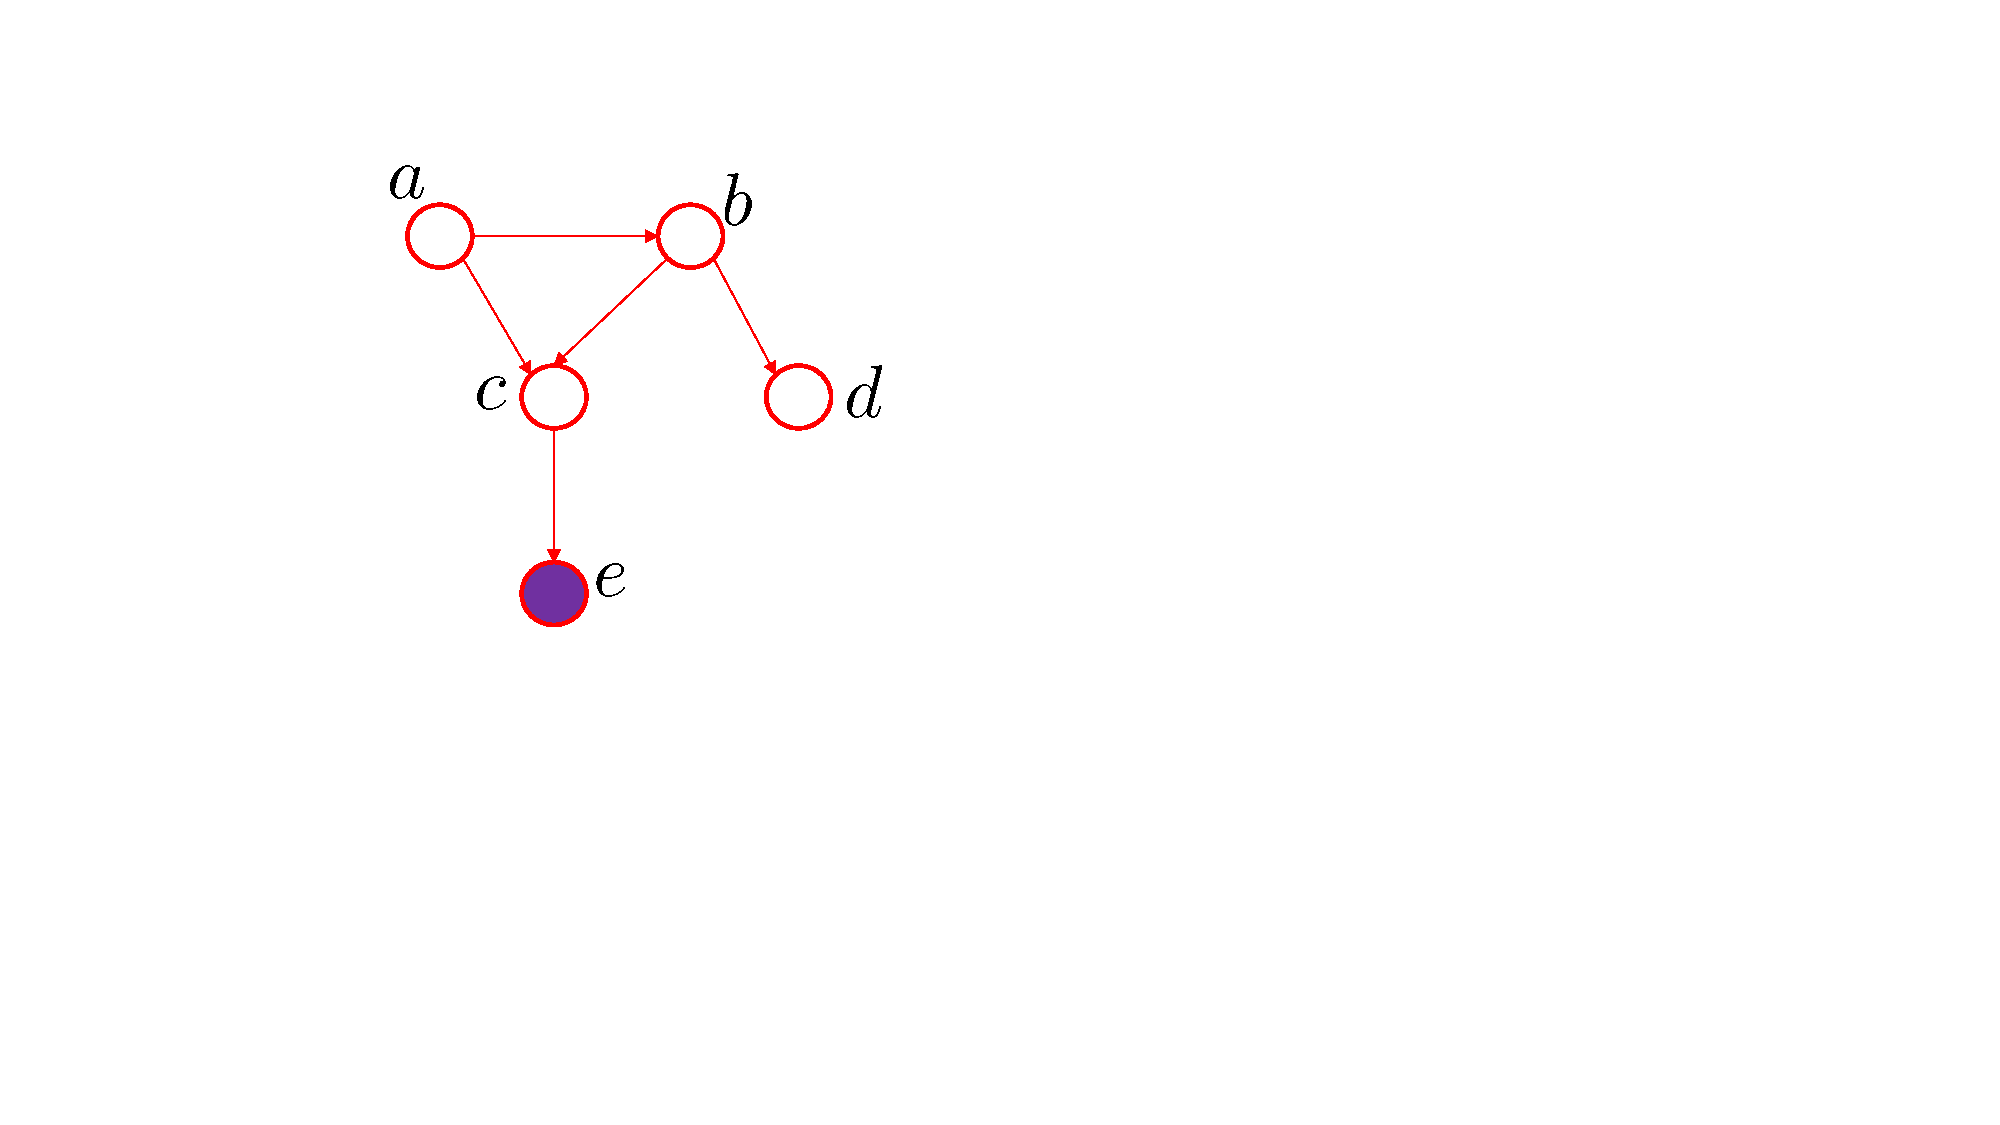
\includegraphics[width=0.1\linewidth]{./fig3_1.pdf} 
	\caption{Model 1.} \label{fig:graph3}
\end{figure}
\begin{figure}[h]
	\centering
	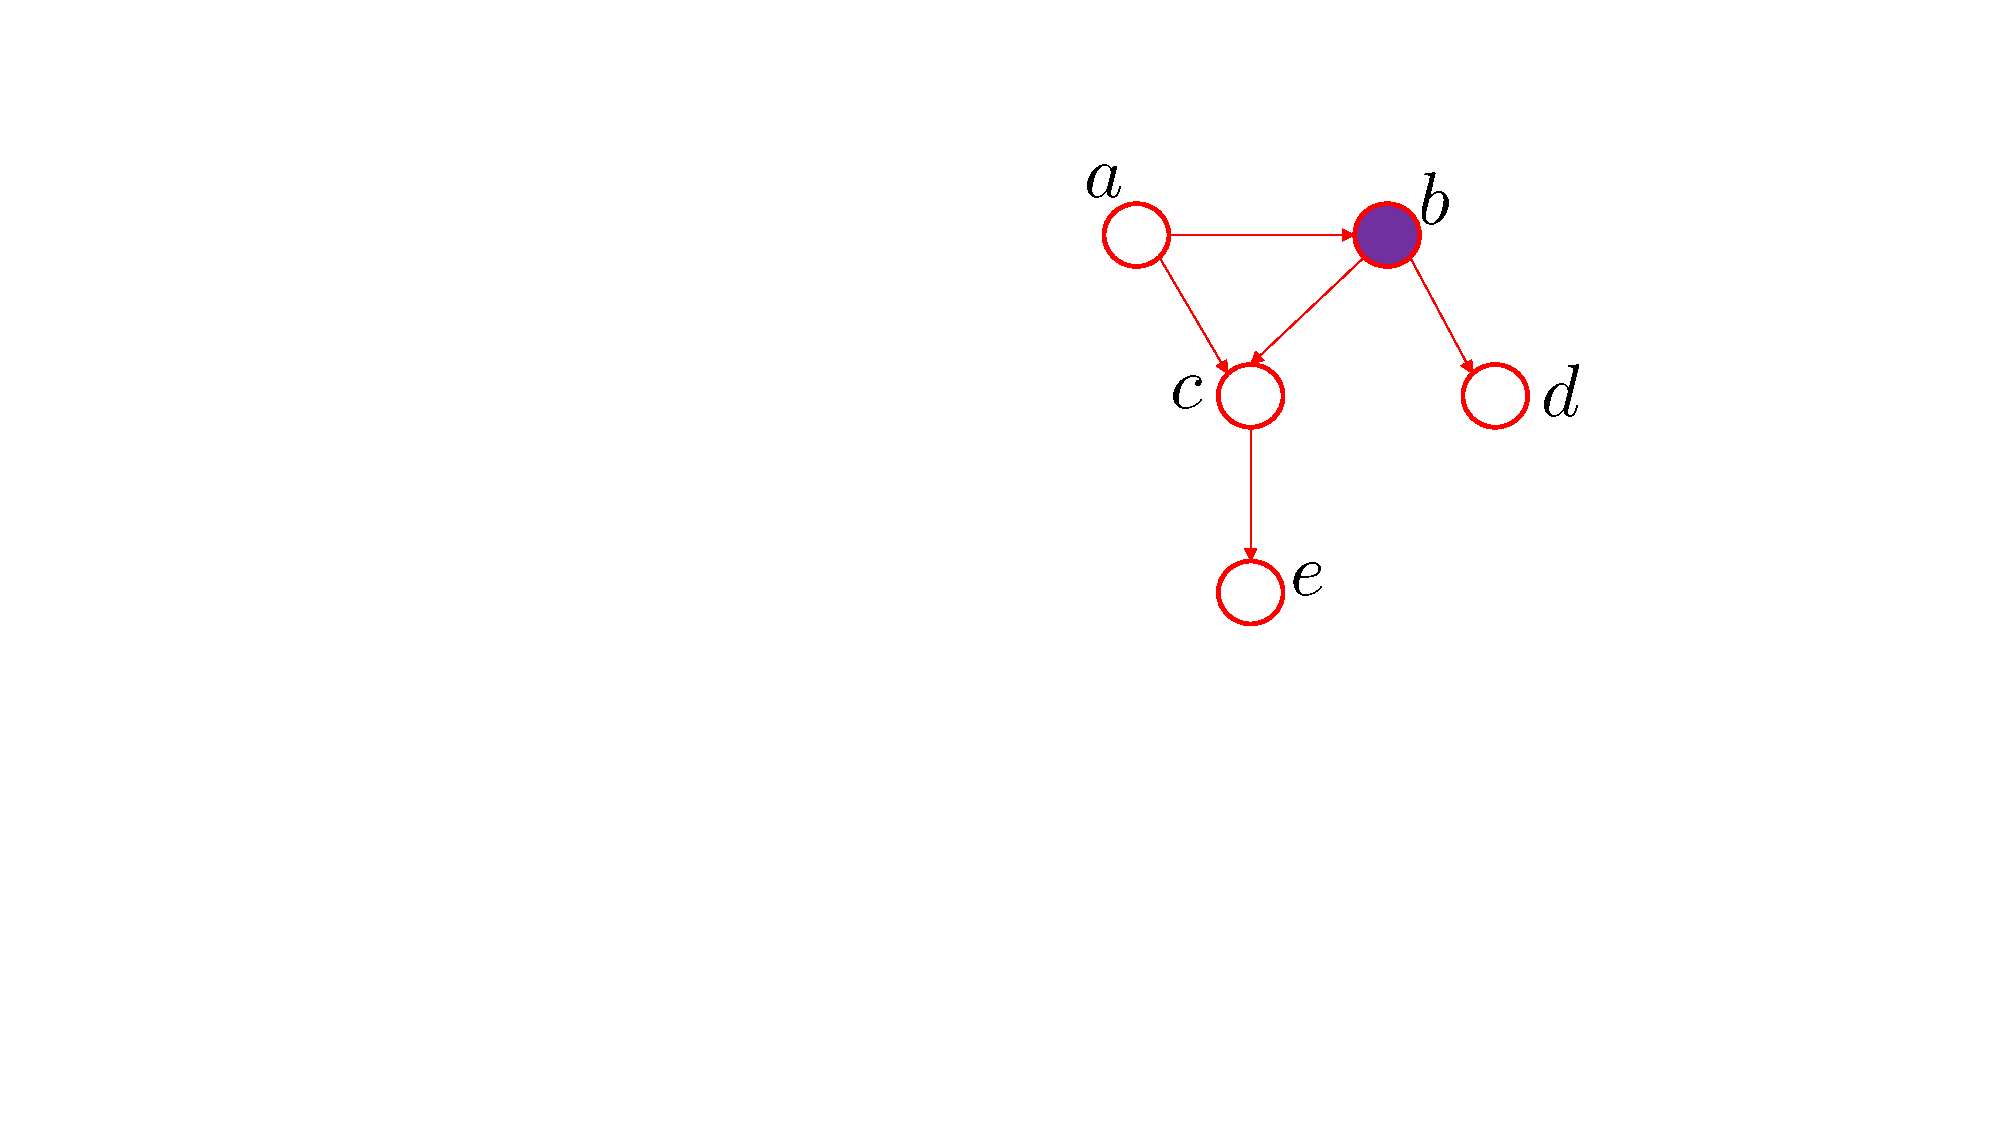
\includegraphics[width=0.1\linewidth]{./fig3_2.pdf} 
	\caption{Model 2.} \label{fig:graph4}
\end{figure}


\item~[15 points] Use d-separation algorithm (Bayes ball) to determine if $a \independent d | e$ in the graphical  model shown in Figure \ref{fig:graph3}, and if $a \independent d | b$ in the graphical model  shown in Figure  \ref{fig:graph4}. \\
{\bf \red Answer: }{\blackblue 
\begin{itemize}
\item $a \not\independent d | e$ in the graphical model shown in Figure  \ref{fig:graph3}.\\
To conclude that  $a \not\independent d | e$, it suffices to find a path from $a$ to $d$ which is not blocked. 
Consider the path $P=acbd$. Nothe that in this path we have two internal vertices $c$ and $b$.
Note that $b$ is a head-to-tail vertex which is not observed and $c$ is a head-to-head vertex with an observed descendant $e$. 
Therefore, this path is not blocked and, in view of d-separation algorithm, $a \not\independent d | e$. 


\item[$\bullet$] $a \independent d | b$ in the graphical model shown in Figure  \ref{fig:graph4}.\\
There are exacltly the two paths $P_1 = abd$ and $P_2= acbd$ from $a$ to $d$ in graph shown in Figure  \ref{fig:graph4}.
In the path $P_1$, the vertex $b$ is in $C=\{b\}$ and also is head-to-tail. Thus, this path is blocked.
In the path $P_2$, the vertex $b$ is in $C=\{b\}$ and also is tail-to-tail. Therefore, this path is also blocked as well.
Since, every path from $a$ to $d$ is blocked, $\{a\}$ is $d$-separated from $\{d\}$ by $\{b\}$, we have $a \independent d | b$.


\end{itemize}


}

\begin{figure}[h]
	\centering
	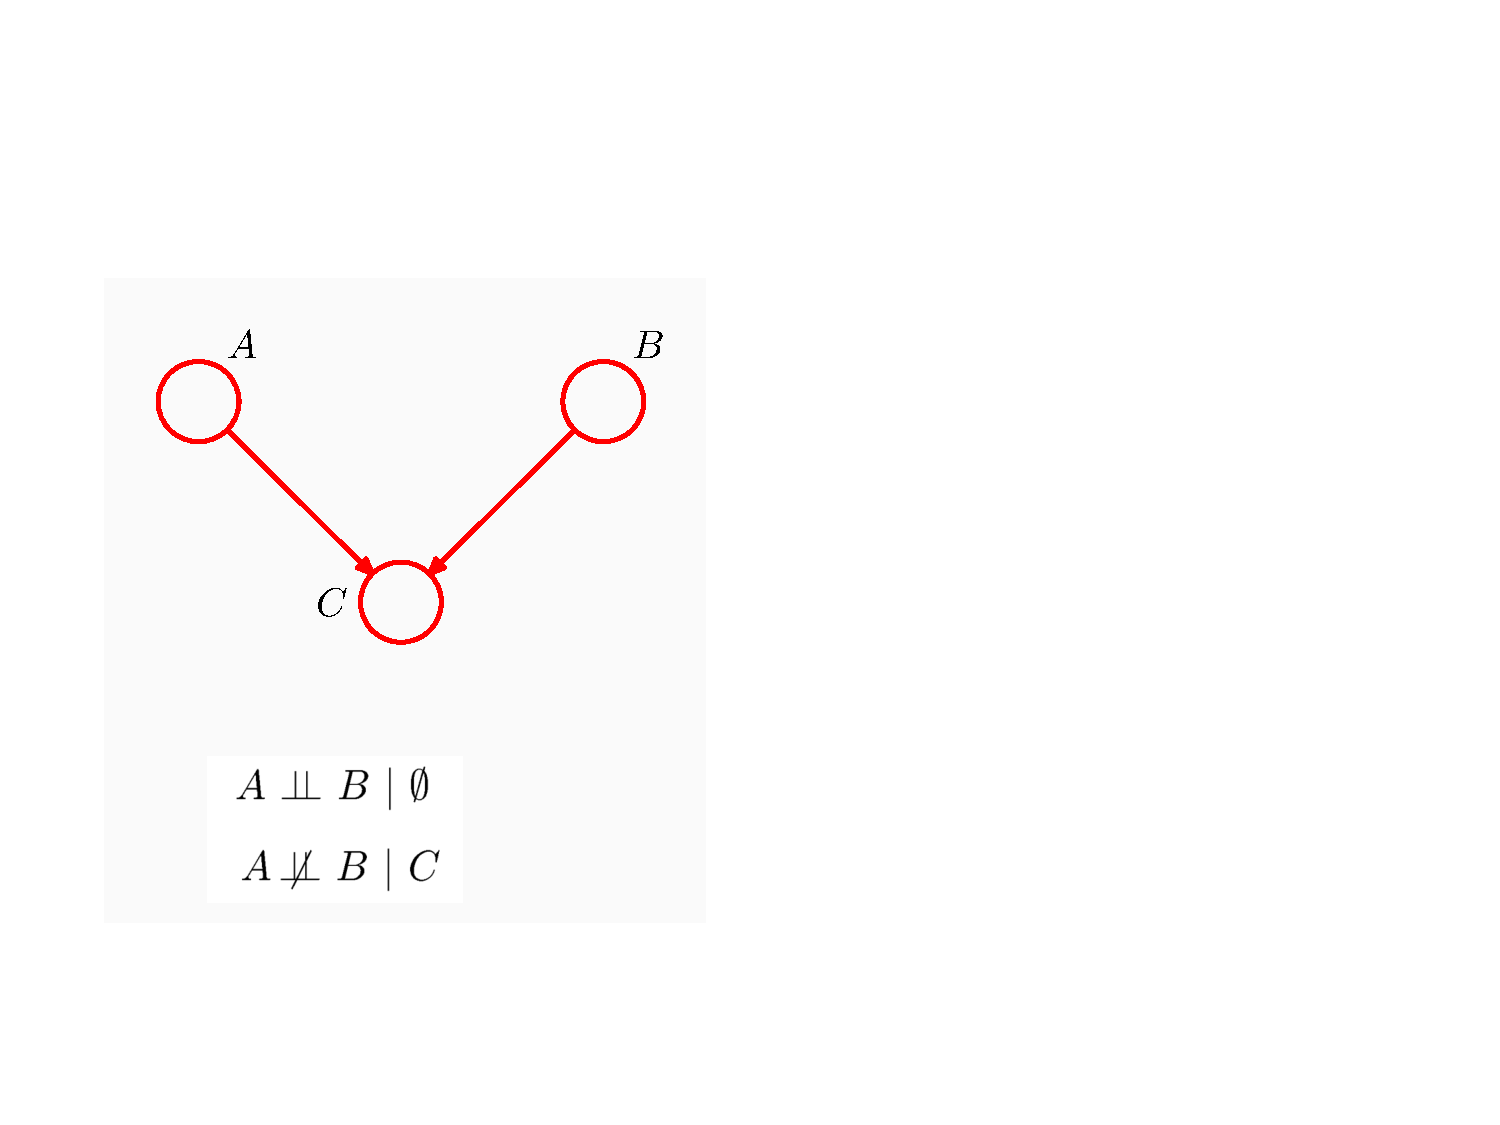
\includegraphics[width=0.2\linewidth]{./fig4.pdf} 
	\caption{Directed.} \label{fig:graph5}
\end{figure}
\begin{figure}[h]
	\centering
	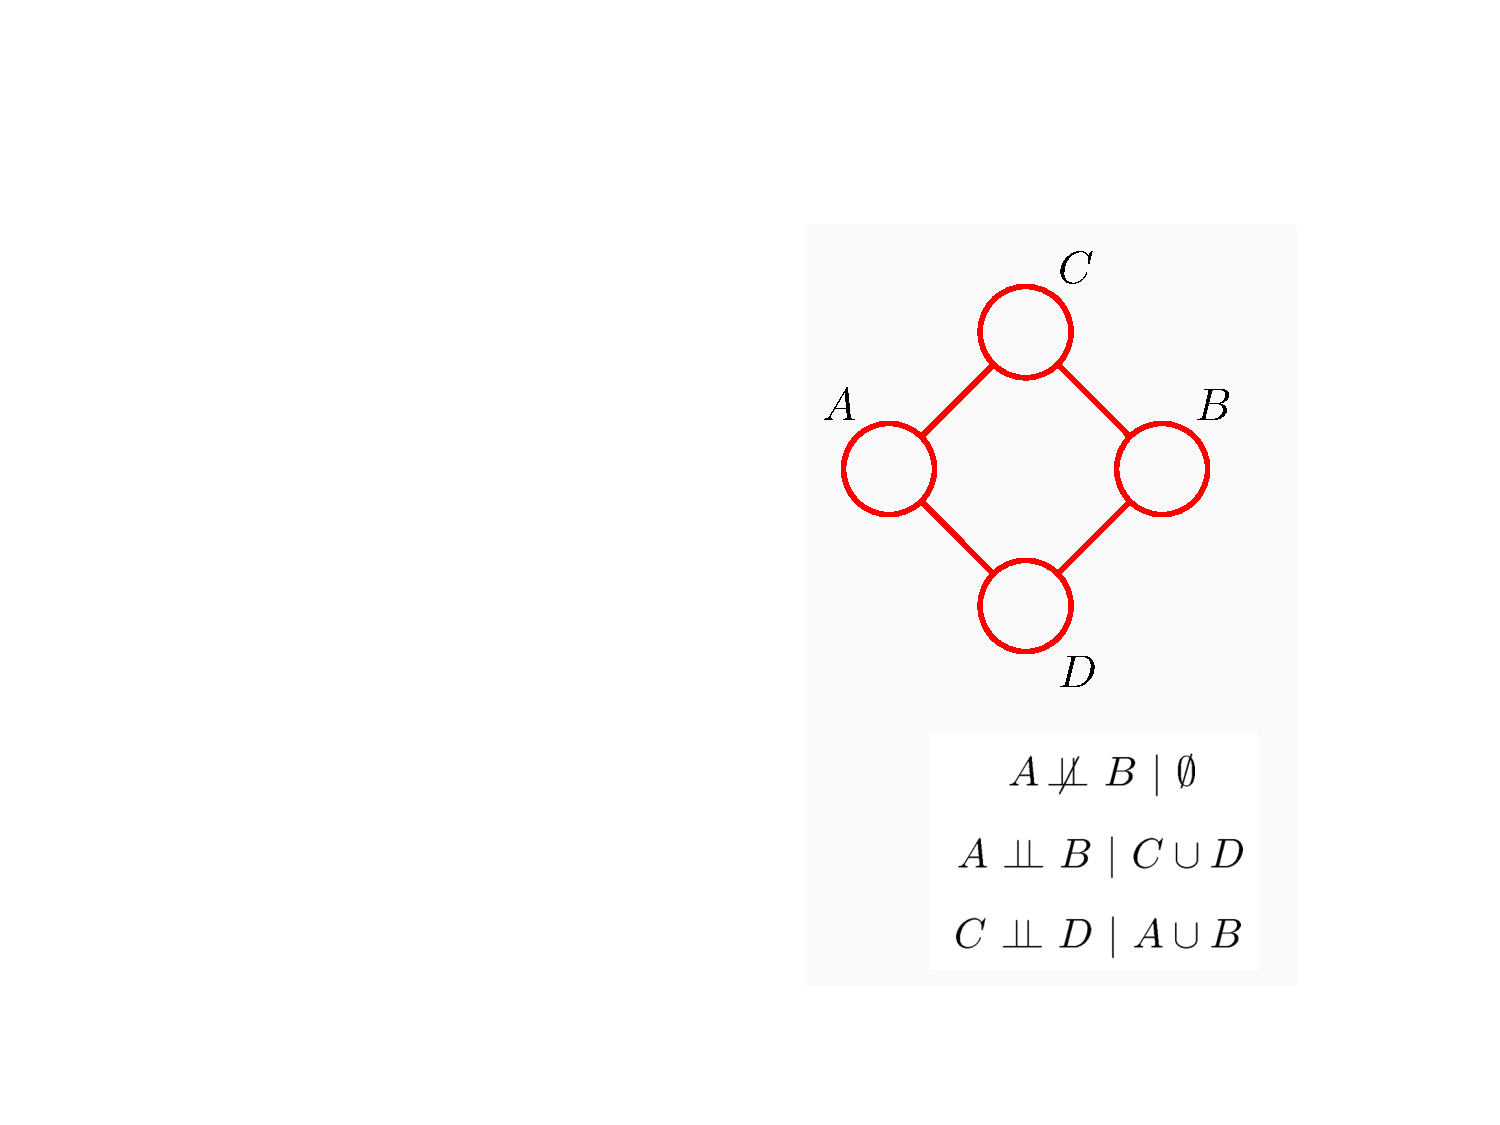
\includegraphics[width=0.2\linewidth]{./fig5.pdf} 
	\caption{Undirected.} \label{fig:graph6}
\end{figure}

\item~[\textbf{Bonus}][20 points] We have listed two examples in the class to show that in terms of the expressiveness (i.e., conditional independence) of the directed and undirected graphical models, there is not a guarantee that who is better than who. 
\begin{enumerate}
	\item~[10 points] Now show that for the directed graphical model in Figure \ref{fig:graph5}, we cannot find an equivalent undirected graphical model to express the same set of conditional independence. \\
{\bf \red Answer: }{\blackblue 
By Figure \ref{fig:graph5},  $p(A,B,C)= P(A)P(B)P(C|A,B)$. Also, we assume that the model in Figure \ref{fig:graph5} perfectly presents $p$. 
For a contradiction, consider an undirected graphical model with the same vertice presenting $p$ perfectly. 
Since, as we have the term $P(C|A, B)$ in $P(A, B, C)$ and $A \not\independent B|C$,  any undirected graphical model expressing the same conditional independence should have verities $A, B$ and $C$ as a clique (fully connected). Therefore, the undirected graphical model should be a triangle with vertices $A, B$, and $C$. In conclusion, there is an edge linking $A$ to $B$ in the undirected graphical model. Note that the undirected graphical model perfectly describes the distribution $p$ which implies $A \not\independent B|\varnothing$, a contradiction. }	
	
\item~[10 points] Show that for the undirected graphical model in Figure \ref{fig:graph6}, we cannot find an equivalent directed graphical model to express the same set of conditional independence. \\
{\bf \red Answer: }{\blackblue 
For a contradiction, assume that there is a directed model that perfectly presents $p(A, B, C, D) = \psi_1(A, C)\psi_2(C, B)\psi_3(B, D)\psi_4(D, A)$.
Since $A\not\independent B|\varnothing$, by $d$-separation theorem, we should have a path from $A$ to $B$ which is not blocked by $\varnothing$. 
So, there is a path from $A$ to $B$ going through $C$ or $D$. Therefore, we have one of the cases in Figure~\ref{fig:graph10}). 
Each cases is denied by the following reason (clockwise).
\begin{itemize}
\item $A\cup B\not \independent|C\cup D$
\item The graph has a cycle.
\item $B\cup D\not \independent|A\cup B$
\item $B\cup D\not \independent|A\cup B$
\end{itemize}
\begin{figure}[h]
	\centering
	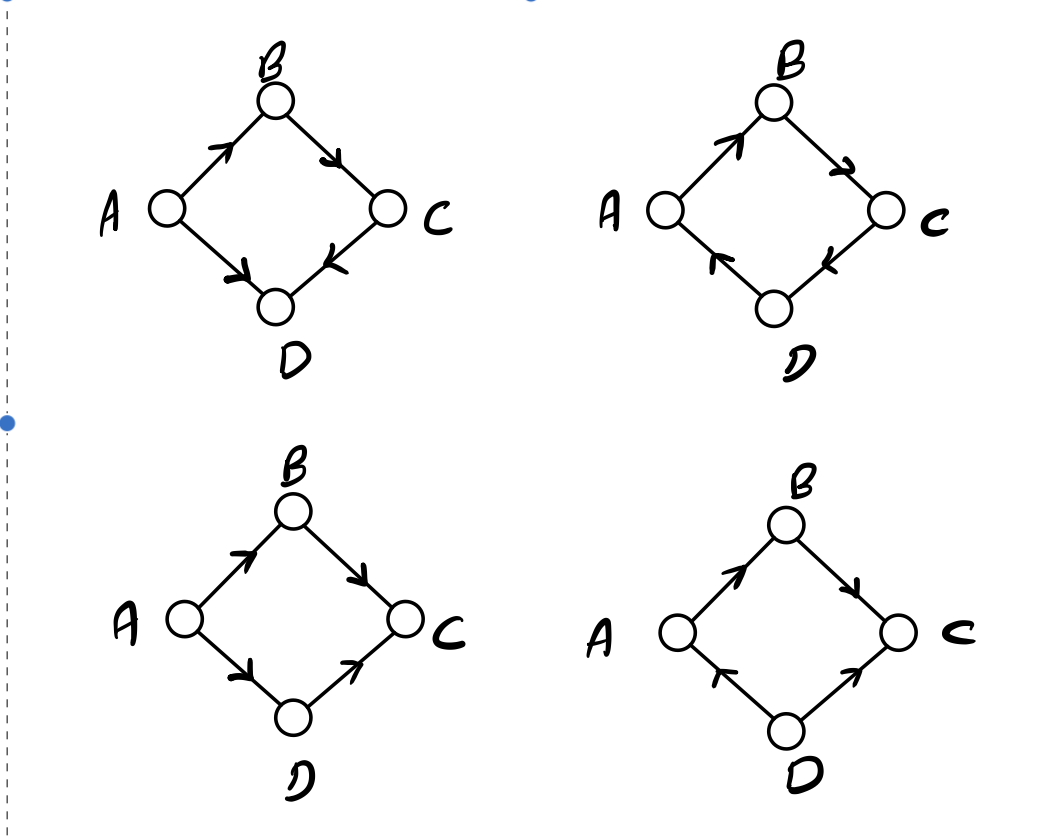
\includegraphics[width=0.4\linewidth]{FigQ10.png} 
	\caption{Directed.} \label{fig:graph10}
\end{figure}

}
\end{enumerate}


\end{enumerate}

\end{document}
